\documentclass{article}

\usepackage{graphicx}
\usepackage{courier}
\renewcommand*\familydefault{\ttdefault} %% Only if the base font of the document is to be typewriter style
\usepackage[T1]{fontenc}

\usepackage[top=1.5in, bottom=1.25in, left=1.5in, right=2in]{geometry}

\thispagestyle{empty}
\pagestyle{empty}

\begin{document}
\begin{figure}
    \centering
    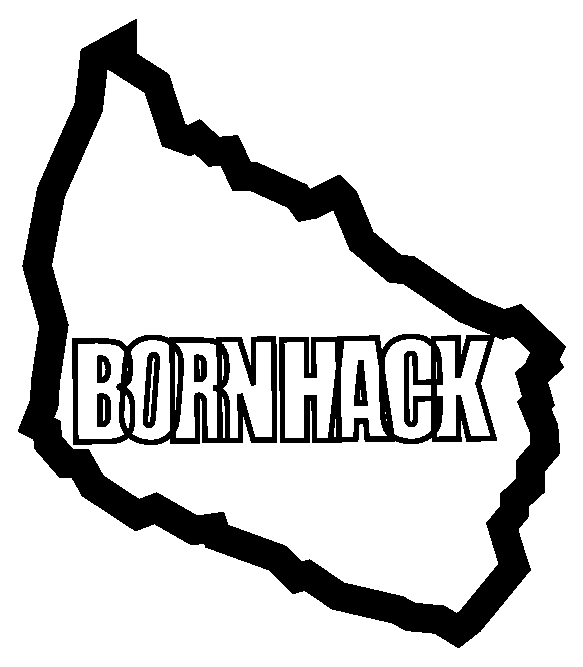
\includegraphics[scale=0.8]{logo.png}
\end{figure}
\noindent {\raggedleft Bornhack is a camp where hackers, makers and people
with an interest in technology come together for a week
to celebrate technology, socialise and have fun.}\\

\noindent {\raggedleft It takes place for the first time from \textbf{August
27 to September 3rd 2016} on the Danish island Bornholm
where we have found the geography as well as the backbone
to make it happen.}\\

\noindent {\raggedleft Bornhack is a participatory event where we expect
people to come up with crazy ideas and help make the
content. We will try to attract interesting people to
give talks and make workshops, but this is just a
setting -- you make the content.}\\

\noindent {\raggedleft We hope you will show your interest by signing onto
our mailing-list as soon as we get it up. In the meantime
you are very much welcome to ask questions and show your
interest on IRC at \textbf{\#bornhack} on \textbf{irc.freenode.net}
such that you can help us understand what \textit{you}
think would be fun to do. This is a new event, so we don't
yet know exactly where this is going -- but give us your
feedback and you can help us form it.}\\

\noindent {\raggedleft We hope you want to be a part of Bornhack -- the Initial
commit}\\


\noindent Sincerely\\
The Bornhack Team

\end{document}
